\documentclass[]{nasa-latex-docs} 

% Preamble Section: %%%%%%%%%%%%%%%%%%%%%%%%%%%%%%%%%%%%%%%%%%%%%%%%%%%%
\usepackage{lipsum}

\docTitle[\docTitleDefault]

\docAbstract[This is an example of using the \acrshort{nasa}-Latex-Docs template. This flexible \latex template is designed to separate content from styling and remove all of the grunt work associated with creating professional documents. This is just a sample of what the output will look like. Please reference the \acrshort{nasa}-Latex-Docs Github wiki for more information and usage guides.]

\begin{filecontents}{mybib.bib}
@online{Template-Guide,
   title = "{GitHub: Nasa-Latex-Docs}",
   year = "2016",
   organization = "NASA",
   url = "https://github.com/nasa/nasa-latex-docs"
}
\end{filecontents} 

\addbibresource{mybib.bib}

\docNomenclature[
$I_{sp}$ & specific impulse \\
$m_0$    & initial total mass, including propellant \\
$m_f$    & final total mass, dry mass \\
$v$      & velocity of the rocket \\
$v_e$    & exhaust velocity \\
]

% Main Document Content: %%%%%%%%%%%%%%%%%%%%%%%%%%%%%%%%%%%%%%%%%%%%%%%
\begin{document}

\section{Introduction}

Please reference the \acrshort{nasa}-Latex-Docs Github wiki\cite{Template-Guide} for more information and usage guides.

\section{Lip Sum Text}

\lipsum[1-4]

\section{Sample Figures}

\ref{fig:NASA_logo} is an example image using the \texttt{figure} environment.

\begin{figure}[H]
   \includegraphics[scale=1.0]{nasa_logo} 
   \caption{This is an Example of Inserting a Figure}
   \label{fig:NASA_logo}
\end{figure}

\subsubsection{Side by Side Figures - One Caption}

\begin{figure}[H]
\begin{subfigure}[b]{0.49\textwidth}
   \centering
   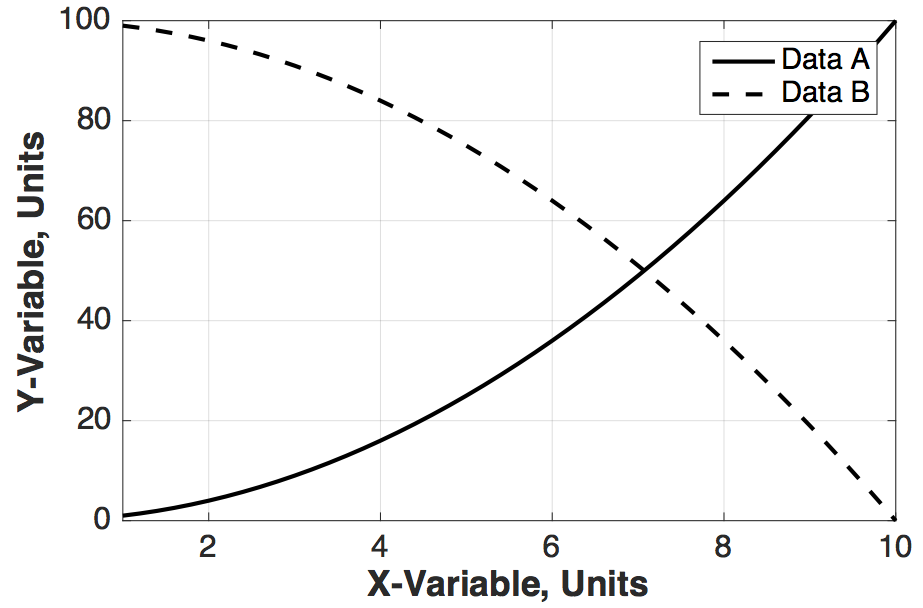
\includegraphics[width = 2.5in]{sample_graph}
   \caption{Left Graph}
   \label{fig:sample_graph_L}
\end{subfigure}
\begin{subfigure}[b]{0.49\textwidth}
   \centering
   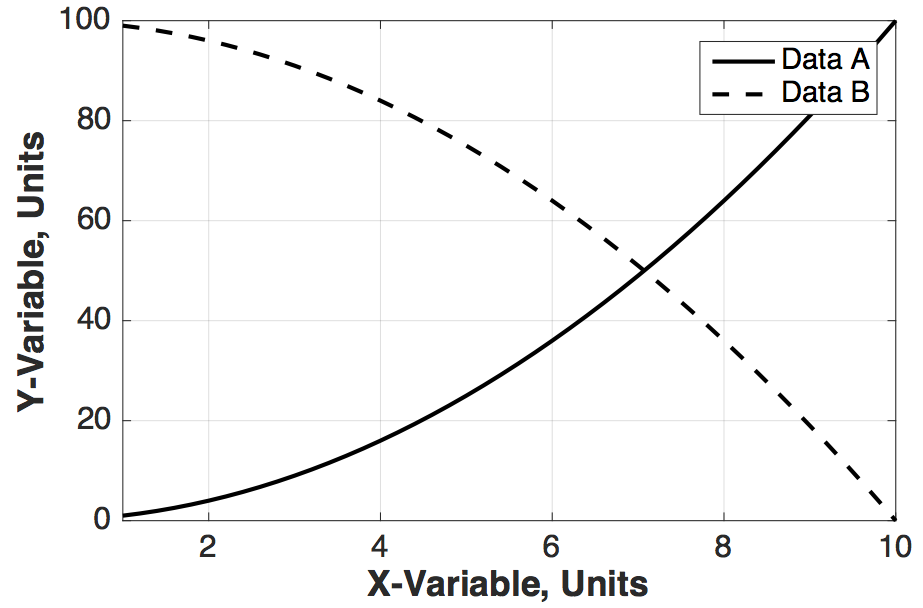
\includegraphics[width = 2.5in]{sample_graph}
   \caption{Right Graph}
   \label{fig:sample_graph_R}
\end{subfigure}
\caption{This is an Example of Inserting Sub-Figures}
   \label{fig:sub_figures}
\end{figure}

\section{Sample Tables}

Creating simple, elegant, tables is easy to accomplish in \latex:

\begin{table}[H]
   \caption{This is an example of a \latex table}
   \label{tab:TabEx}
   \begin{tabular}{lccr}
      \toprule[\heavyrulewidth]
      \toprule[\heavyrulewidth]
      \textbf{Main Item 1} & \textbf{Main Item 2} & \textbf{Main Item 3} \\
      \midrule
      Value Item 1 & Value Item 2 & Value Item 3 \\
      Value Item 1 & Value Item 2 & Value Item 3 \\
      \bottomrule[\heavyrulewidth]
   \end{tabular}
\end{table}

\subsection{Table with Multiple Columns}

To create multiple columns, use the \texttt{\textbackslash multicolumn} command:

\begin{table}[H]
   \caption{\latex table with a multiple column entry}
   \label{tab:TabEx2}
   \begin{tabular}{lccr}
      \toprule[\heavyrulewidth]
      \toprule[\heavyrulewidth]
      \textbf{Main Item 1} & \textbf{Main Item 2} & \textbf{Main Item 3} \\
      \midrule
      \multicolumn{2}{c}{Multiple Column Entry}  & Value Item 3 \\
      Value Item 1 & Value Item 2 & Value Item 3\\
      \bottomrule[\heavyrulewidth]
   \end{tabular}
\end{table}

\subsection{Table with Multiple Rows}

To create multiple rows, use the \texttt{\textbackslash multirow} command:

\begin{table}[H]
   \caption{\latex table with a multiple row entry}
   \label{tab:TabEx3}
   \begin{tabular}{lcc}
      \toprule[\heavyrulewidth]
      \toprule[\heavyrulewidth]
      \textbf{Main Item 1} & \textbf{Main Item 2} & \textbf{Main Item 3} \\
      \midrule
      \multirow{2}{*}{Multiple Row Entry} & Value Item 2 & Value Item 3 \\
      & Value Item 2 & Value Item 3 \\
      \bottomrule[\heavyrulewidth]
   \end{tabular}
\end{table}

\section{Sample Equations}

\latex is fantastic for creating equations, as seen in \ref{eq:tsiolkovsky}. \Ref{eq:tsiolkovsky} is the Tsiolkovsky rocket equation describing the basic principles of rocket motion. \latex can also be used for in-line equations. In this equation the exhaust velocity, $v_e$, can be expressed as $v_e=I_{sp}g_0$ where $I_{sp}$ is the specific impulse and $g_0$ is the standard gravity.

\begin{equation} \label{eq:tsiolkovsky}
   \Delta v = v_e\ln\frac{m_0}{m_f}
\end{equation}

\section{Sample Lists}

% \latex provides several environments for creating lists.

\subsection{Bulleted List (\texttt{itemize} environment)}

\begin{itemize}
  \item The first item
  \item The second item
  \item The third item
\end{itemize}

\subsection{Enumerated List (\texttt{enumerate} environment)}

\begin{enumerate}
  \item The first item
  \item The second item
  \item The third item
\end{enumerate}

\subsection{Description List (\texttt{description} environment)}

\begin{description}
  \item[First:] The first item
  \item[Second:] The second item
  \item[Third:] The third item
\end{description}

\subsection{Nested List}

List environments can also be nested and combined:

\begin{enumerate}
   \item The first item
      \begin{itemize}[topsep=0pt]
         \item The first sub-item
         \item The second sub-item
      \end{itemize}
   \item The second item
   \item The third item
\end{enumerate}

\section{Sample TikZ Graphics}

\usetikzlibrary{arrows}
\tikzstyle{int}=[draw, fill=blue!20, minimum size=0.5in]
\tikzstyle{init} = [pin edge={to-,thin,black}]

\begin{figure}[H]
      \begin{tikzpicture}[node distance=2in,auto,>=latex']
               \node [int, pin={[init]above:$v_0$}] (a) {$\frac{1}{s}$};
               \node (b) [left of=a,node distance=1in, coordinate] {a};
               \node [int, pin={[init]above:$p_0$}] (c) [right of=a] {$\frac{1}{s}$};
               \node [coordinate] (end) [right of=c, node distance=1in]{};
               \path[->] (b) edge node {$a$} (a);
               \path[->] (a) edge node {$v$} (c);
               \draw[->] (c) edge node {$p$} (end);
      \end{tikzpicture}
      \caption{Example Image Using TikZ Package}
      \label{fig:block_diagram}
\end{figure}

\section{Sample Code Listings}

\lstinputlisting[caption=Example C Code Listing, label=cExample,language=C, numbers=left]{sample_C.c}

\end{document}
% End of Document %%%%%%%%%%%%%%%%%%%%%%%%%%%%%%%%%%%%%%%%%%%%%%%%%%%%%%